
\section{Control}

\subsection{intro}
Today, this kind of operation is done by maneuvring the vehicle to a position where the manipulator is within reach of the hot stab. Once the desired vehicle position is reached, the vehicle is kept stationary by using dynamical positioning, and another operator operates the manipulator arm to do insert the hot stab. The manipulator is normally controlled through a master-slave configuration,\footnote{A master-slave configuration is a control method where an operator moves a replica of the real manipulator. The obtained angles of the replica is then used by the motion control of the manipulator to obtain the same pose as the replica.} 
or through controling the rates of the joints directly. Both these methods suffer from the following drawbacks:

\begin{itemize}
	\item The operator is dependant on high video feedback with very low latency in order to make the correct adjustments of the manipulator.  
	\item Two operators are normally required, one for the vehicle and one for the manipulator arm.
	\item One has to switch between maneuvring the vehicle and the manipulator, even for tasks that are fairly close to eachother, potentially using more energy then required by the task itself. 
	\item Interaction with the environment is difficult due to latency in force feedback from the manipulator, and difficulty in estimating the forces caused by the interaction.
\end{itemize}
One of the objectives of the control strategy is to keep the human operator out of the control loop as much as possible. This makes the system less dependant on high speed telemetry which is important when operating nontethered vehicles, making it possible to control them from a great distance. 
The proposed control structure is based on controlling the motion of the end effector seen from the end effector frame \frame{ee}. Kinematically this will be done by an inverse kinematic strategy mapping the end effector velocities 
to joint, and vehicle velocities, which will be discussed later. This gives the operator the opportunity to ``fly'' the end effector, without dealing with the rest of the manipulator or the vehicle, as this is being managed locally by the control system. 
Lets now identify the main states of operation of the UVMS, which is useful when designing the control system. 

\begin{itemize}
	\item Transport. This state represent the relatively long distance transport of the UVMS to and from a location where it operates, or when doing inspections of e.g. pipelines. This state requires relatively low accuracy in guidance and is typically done by maneuvering the vehicle only. This can be employed by a classical path following guidance scheme. (See e.g. \cite{fs})  
	\item Repositioning between operation points. In this state, the operator or a path following guidance system will ``fly'' the end effector from one operation point to another, covering relatively short distances. In this state the end effector is controlled and adjusted by an operator controlling the velocities of the end effector.
	\item End effector interaction. The manipulator is used to interact with the environment, for example in a hot stab operation. In this state, high accuracy is required, and should be automatically regulated locally, giving the operator control over the directions of no contact.
\end{itemize}
Before continuing with the force control, a discussion of path following and accuracy is needed. In the two first states the vehicle or the end effector is following a path given by an operator, a path following guidance scheme, or both. The accuracy of the position relative to the desired path is then controlled by the operator through video feedback, or through a guidance system (such as the LOS Guidance Law. See e.g. \cite{fs}). In both cases the guidance is done at a relatively low bandwith, making the path following prone to disturbances, and hence causing the actual path to deviate from the desired path. It is assumed that the reference given to the low level motion control is given as the generalized and quasi velocities of the joints and vehicle. When interacting with the environment the position of the end effector needs to be position controlled at a relatively high bandwidth. This is important in order to be robust to disturbances, and avoid undesired forces on the end effector. To maintain a high bandwidth on the position control, it is recommended that this is done locally, keeping the human out of the position control loop.

A generalized control strategy for the two last states above will now  be proposed, and will later be specified for a hot stab operation. The overall control structure is illustrated in Fig. \ref{fig:control_structure}. Lets now define the desired path given by the operator as $\bs V_{ee,0}$ and $\bs \eta_{ee,0}$. In the second state of operation, only the desired velocity $\bs V_{ee,0}$ is used to specify the desired trajectory. The high bandwidth motion of the end effector is given as $\bs V_{ee,c}$. In the second state we use that 
$$\bs V_{ee,0} = \bs V_{ee,c} $$ 
In the case of the second state of operation the desired velocities of the end effector is mapped, through the inverse kinematics, to reference velocities $\bs \zeta_{c}$ used in the low level motion control.
\begin{figure}[h!]
	\centering
	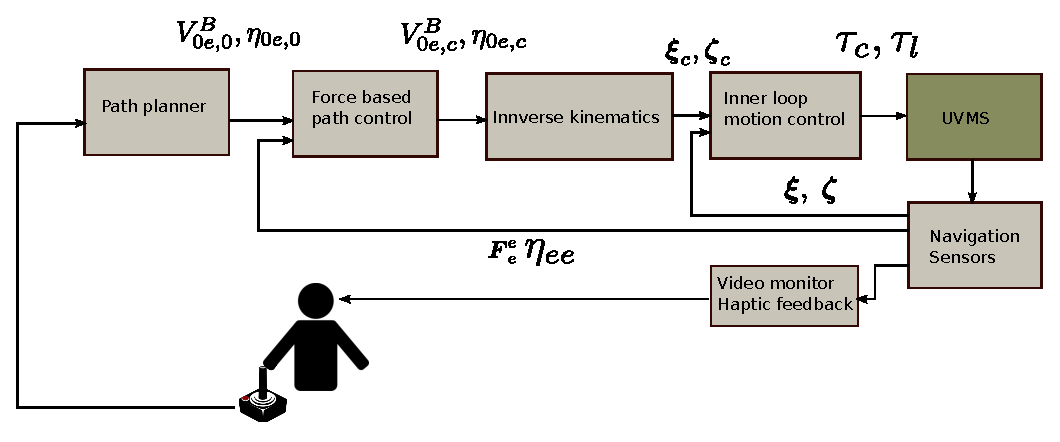
\includegraphics[scale=0.9]{./figures/control_structure.eps}
	\caption{Control structure}
	\label{fig:control_structure}
\end{figure}
In the third state of operation accurate position control is essential, and another approach is therefor proposed specifically for a hot stab operation in the test case below. 

\subsection{Test Case: Semi Autonomous Hot Stab Operation}
A hot stab is a typical operation done by ROV's on subsea installations, which gives the opportunity to connect and disconnect different hydraulic components. 
The hot stab operation is in many ways analogous to the ``peg-in-hole'' problem which is widely studied in robotics litterature. The terms peg and hole will from now on refer to the hot stab tool, and the hole it is inserted into. 
Today, hot-stab is typically done by an operator controlling all of the degrees of freedom of the end effector, or directly in the joint space of the manipulator. This leads to difficulty in putting the peg in the hole, ecpecially 
with large delays in the human-UVMS-loop. 
The proposed strategy in this section is to lock most of the degrees of freedom to position set-points, and let the operator control a minimal set of DOFs. A fuzzy rule will handle the position set-points when the end effector is in 
contact with the environment. The concept is illustrated in Fig. \ref{fig:hot_stab2}.


\begin{figure}[h!]
	\centering
	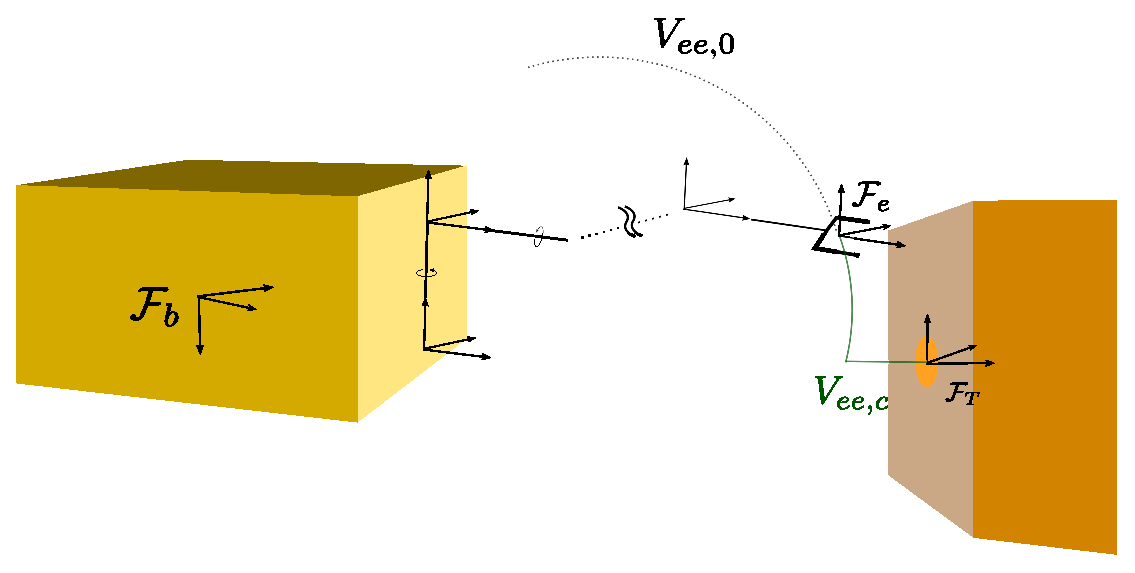
\includegraphics[scale=0.7]{./figures/uvms_hot_stab2.eps}
	\caption{Illustration of the UVMS in the transition between an operator ``flying'' the end effector according to $\bs V_{ee,0}$, and being position controlled in the $z,y,\theta $ and $ \psi$ direction in order to align with the task frame \frame t}
	\label{fig:hot_stab2}
\end{figure}
Further the sets $C$ and $NC$ are defined as

\begin{align*}
	C&=\{y_{ee},z_{ee},\theta_{ee},\psi_{ee}\} - \text{Compliant pose variables}
	\\
	NC&=\{x_{ee},\phi_{ee}\} \; \; \; - \; \text{ Non-Compliant pose variables}
\end{align*}
Where the axes above refer to the axes of \frame{ee}. Further, the set-points $\bs \eta_{ee,0}$, given by the operator are good approximations to the pose of \frame{t} given in the inertial frame. Without loss of generality \frame{t} will be used as the inertial frame, and therefor the set-points are given as  
\begin{align}
C \subseteq	\bs \eta_{ee,0}=0
	\label{eq:subset}
\end{align}
A simple outer loop control law is proposed in order to assign a proper commanded velocity variables to the inverse kinematic control, and furhter, to the low level motion control

\begin{align}
	\bs V_{ee,c} &= \beta \left( \bs F_{ee} \right) \bs K_{1}\bs V_{ee,0} + \alpha \left( \bs F_{ee} \right) \bs K_{2} \tilde{\eta}_{ee} 
	\label{eq:control_law1}
	\\
	\alpha, \beta &\in \left[ 0,1\right]
	\\
	\bs K_{1},\bs K_{2}&\in \Real{6 \times 6} \\
	\tilde{\bs \eta}_{ee,0}&= \bs \eta_{ee,0} - \widehat{\bs \eta}_{ee}
\end{align}
Where $\widehat{\bs \eta}_{ee}$ is the estimated or measured pose of the end effector. The matrices $\bs K_{1}$ and $ \bs K_{2}$ are selection matrices, which selects the variables corresponding to $C$ and $NC$. $\bs K_{2}$ also weighs the contribution of the pose error.  

\begin{align}
	\bs K_{1} =\left[\begin{matrix}{}1 & 0 & 0 & 0 & 0 & 0\\0 & 0 & 0 & 0 & 0 & 0\\0 & 0 & 0 & 0 & 0 & 0\\0 & 0 & 0 & 1 & 0 & 0\\0 & 0 & 0 & 0 & 0 & 0\\0 & 0 & 0 & 0 & 0 & 0\end{matrix}\right]
	\label{eq:k1k2} \; , \; 
\bs K_{1} &=
\left[\begin{matrix}{}0 & 0 & 0 & 0 & 0 & 0\\0 & k_{22} & 0 & 0 & 0 & 0\\0 & 0 & k_{23} & 0 & 0 & 0\\0 & 0 & 0 & 0 & 0 & 0\\0 & 0 & 0 & 0 & k_{25} & 0\\0 & 0 & 0 & 0 & 0 & k_{26}\end{matrix}\right]
\end{align}
And the scalar functions $\alpha$ and $\beta$ are veighting the different terms in \eqref{eq:control_law1} based on a fuzzy rule described later. Taking $\alpha = \beta = 1$, the control law in \eqref{eq:control_law1} acts as a PI controller on the end effector velocity $\bs V_{ee}$. Where the pose is regarded as the integral of the velocity. Although this is not true in general, since the angular velocities $p_{ee}, q_{ee}$ and $r_{ee}$ in  $\bs V_{ee}$ are quasi-velocities, it can be shown that it is a good approximation close to the end effector pose $\phi_{ee} = \theta_{ee}=\psi_{ee}=0$. The approximation of transformation matrix $\bs T$ from body velocities to euler angle rates, for small angles $\delta \phi, \delta \theta$ and $\delta \psi$ is given in \cite{fs} as

\begin{align}
	\bs T(\delta \bs \eta_{2}) &\approx \begin{bmatrix} 1 & 0 & \delta \theta \\ 0 & 1 & -\delta \phi \\ 0 & \delta \phi & 1 \end{bmatrix}	
	\label{eq:linearized-transformation}
	\\
	\bs T(\delta \bs \eta_{2}) \big|_{\eta_{2}=0} &\approx \bs I_{3 \times 3}
	\label{eq:linearized-transformation2}
	\\
	\dot{\bs \eta}_{ee}&\approx\bs T(\delta \bs \eta_{2}) \begin{bmatrix} p \\ q \\ r\end{bmatrix}
	\\
	\Rightarrow \dot{\bs \eta}_{ee}&\approx \begin{bmatrix} p \\ q\\  r\end{bmatrix}
\end{align}
It is important to notice that the euler representation gives singularities for certain configurations. Therefor, in a robust implementation, quaternions could be used instead. For the purpose of analysis, however, the euler angles have a more intuitive interpretation, and will be used throughout this section.
Besides acting as a PI controller, the last term in \eqref{eq:control_law1} can also be seen as a path correction term, correcting the velocity $\bs V_{ee,0}$ when deviating from the desired path. When the end effector is in the free flying state, this path correction is done by the operator, correcting the velocity based on observed deviations through e.g. video feedback. 

It is reasonable to assume that the hot-stab system is designed so that it allows a slight error of the positions in $C$, for instance through making the insertion point bigger than the size of the peg, and gradually decreasing in size to make the peg fit. If the $C$ -positions are commanded correctly relative to \frame t the simple PI design of \ref{eq:control_law1} with $\alpha=\beta=1$ is sufficient. However, small deviations can occure, either a result of the low level control loop's inability to track the commanded velocity, or by a slight misalignment of the task frame \frame t relative to the physical task. As a result of this, the set points in $C \subseteq \bs \eta_{ee,0}$ can cause the end effector to be commanded (through $\bs V_{ee,c}$) to a set point causing collision with the rigid structure of the environment. This can be seen from \eqref{eq:control_law1}, where a nonzero $\bs K_{2}\tilde{\bs \eta}_{ee}$ commands the end effector to keep a velocity in a direction blocked by the rigid environment.

More generally, the directions controlled purely by velocity will be more compliant to interaction with the environment, as long as the desired velocity is zero. Although an interaction with the environment causes the end effector to be slightly off the planed velocity trajectory, it will only regulate the velocity to 0, and not try to push on the environment due to a position offset. If the position correction term is used, (corresponding to a nonzero $\alpha$)
the end effector will be commanded to push on the environment, if the set-points are slightly off the free motion path. A fuzzy tuning rule for $\alpha$ is therefor proposed to stop the position correction term in \eqref{eq:control_law1} when a the magnitude of the force $\bs F_{ee}$ has reached a certain threshold. 


Let the the p-norm of $\bs F_{ee}$ for $p=2$ be denoted $$F_n=||\bs F_{ee}||_{2}$$ The scalar function $F_{n}$ is then a measure of the total amount of force acting on the end effector. The proposed tuning of $\alpha$ is listed in algorithm \ref{alg:alt1} 

\begin{algorithm}
	\caption{Algorithm converts SOP equation to RPN \label{alg:alt1}}
\begin{algorithmic}[1]
\REQUIRE Initialize a $stack$ and a $queue$
\FOR{$token$ in $SOP$}
    \IF{$token$ is a label}
        \STATE add $token$ to $queue$
    \ELSIF{$token$ is + or *}
        \IF{$token$ is + and top of $stack$ is *}
            \STATE pop the top of $stack$ to $queue$
        \ENDIF
        \STATE push $token$ onto $stack$
 
    \ELSIF{$token$ is (}
        \STATE push $token$ onto $stack$
    \ELSIF{$token$ is )}
        \STATE keep popping operators from $stack$ to $queue$ until sees (
    \ELSE
        \STATE error, exit
    \ENDIF
\ENDFOR
\STATE No more $token$ to consume, pop operators from $stack$ to $queue$
\RETURN $queue$
\end{algorithmic}
\end{algorithm}
















\subsection{Motion Control}
The inner loop of the motion control is outside the scope of this text. For modelling and simulation purposes however, a control strategy based on feedback linearization is proposed, and implemented in SIMULINK in order to 
simulate the force control and the inverse kinematics. To simplify the implementation and analysis we use the model of the UVMS from \eqref{eq:dyn_with_current} split the input $\bs \tau$ into a cancelling term $\bs \tau_c$ and a 
linear control term $\bs \tau_l$ and use $\bs \tau_c$ to cancel out all the nonlinearities and terms including the current. The interaction forces are also left out for now, yielding

\begin{align}
	\bs M(\bs q)_{RB}\zetadotb = \bs \tau_l
	\label{eq:linearized_feedback}
\end{align}








\subsection{Force Control 2}
\begin{figure}[h!]
	\centering
	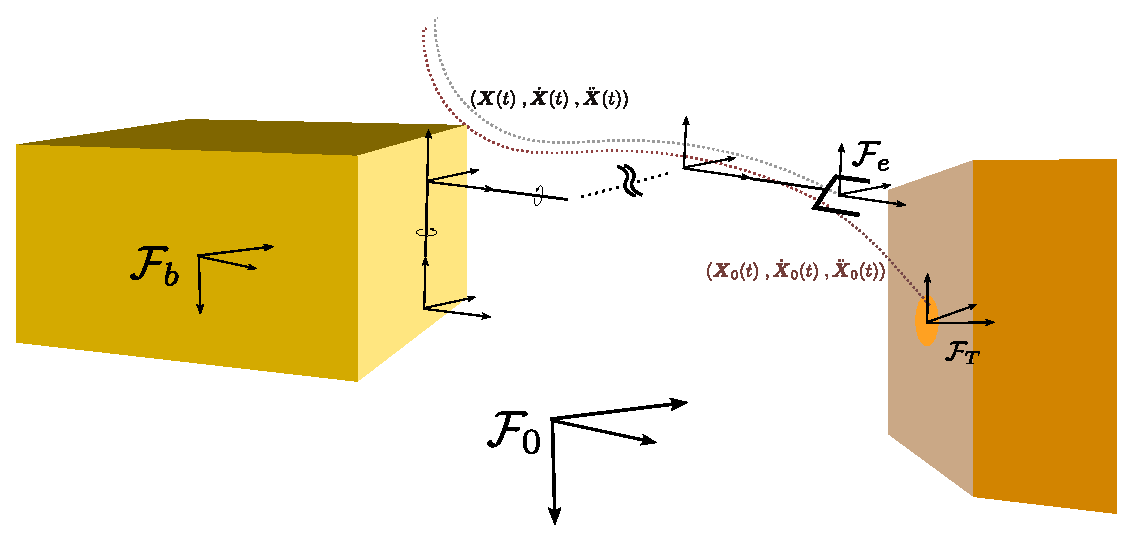
\includegraphics[scale=0.7]{./figures/uvms_kinematics_force.eps}
	\caption{Frames of the UVMS with the inertial and task frame}
	\label{fig:uvms_force}
\end{figure}
The force control is analyzed in the task space, as observed by the end effector, and we can define the forces acting upon the manipulator due to contact with the environment 
\begin{align}
	\bs F_e^e&=\begin{bmatrix} f_x & f_y & f_z & m_x & m_y & m_z \end{bmatrix}
	\label{eq:force_force}
\end{align}
$\bs F_e^e$ is therefor the same as $\bs F$ defined in \eqref{eq:jacobian_force} and can therefor be mapped into the joint the general forces $\taub$ by the transpose jacobian
\begin{align}
	\taub&=(\jb{ge}{B})^T\bs F_e^e
	\label{eq:jacobian-force2}
\end{align}
Let the translational part of the trajectory of the end effector be defined as

\begin{align}
	\bs X(t) \; , \; \dot{\bs X}(t)\; , \; \ddot{\bs X}(t)	
	\label{eq:ee_traj}
\end{align}
Which gives the position, velocity and acceleration of the end effector relative to the task frame \frame T, illustrated in Fig. \ref{fig:uvms_force}. Further we will define a nominal trajectory which represents the planned 
trajectory, given by a path plan algorithm and/or an operator

\begin{align}
	\bs X_0(t) \; , \; \dot{\bs X}_0(t)\; , \; \ddot{\bs X}_0(t)	
	\label{eq:nominal_force}
\end{align}
We can then model the force due to interaction, when the end effector is in contact with the environment, \cite{impedance_stability}

\begin{align}
	\bs F&=\bs K(\bs X - \bs X_0) + \bs B(\dot{\bs X} - \dot{\bs X}_0) + \bs J(\ddot{\bs X} - \ddot{\bs{X}}_0)
	\label{eq:ee_impedance1}
\end{align}
The nominal path can then be interpreted as the no contact path. The constants $\bs K$, $\bs B$ and $\bs J$ can then be regarded as the desired stiffness, damping and inertia of the end effector in contact with the environment. The impedance defined in \eqref{eq:nominal_force} can then be obtained either by direct force control, or it can be used to adjust the path of the endeffector, relying on an inner position control loop. In this paper the latter will be discussed. \cite{impedance_stability} proposes an adjustment vector $\bs X_a$ which is a result of filtering $\bs F$ through a second order low pass filter. We will, for the sake of simplicity only consider diagonal $\bs K$, $\bs B$ and $\bs J$ matrices, so that the forces are decoupled. We can then write the adjustment of the commanded trajectory as

\begin{align}
	\bs X_{a,i}(s)&= \frac{1}{(K_i+ B_is+ J_is^2)} f_i(s) \; , \; i=x , y , z 
	\label{eq:x_adjusted}
\end{align}
$\bs X_a$ can then be seen as a perturbation from the nominal path due to the desired impedance, as defined in \eqref{eq:ee_impedance1}.  The commanded trajectory $\bs X_c$ that is used as the input for the motion control loop can then be written as
\begin{align}
	\bs X_c&= \bs X_0 + \bs X_a
	\label{eq:controlled_traj}
\end{align}
If the inner control loop manages to track $\bs X_c$ perfectly, the impedance between the environment and the end effector is described by \eqref{eq:ee_impedance1}. In practice it is very difficult to track the commanded trajectory perfect, and one must therefor analyze the system further in terms of robustness. The inner control loop is outside the scope of this paper, and we will for now tolerate a small deviation between the commanded trajectory, and the actual trajectory. Designing the impedance based position adjustment whithout the knowledge of the error dynamics of the inner control loop gives a flexible and modular design, but demands a possibly higher robustness, to match the unknown uncertainties 

In the development of a force control strategy one have to take into consideration the challanges in operating an ROV-manipulator underwater. In many cases, exact position tracking is difficult, also the unstructured environment
makes it difficult to obtain good hybrid impedance/position control. It is therefor important to develop strategies and algorithms that does not demand high knowledge of the environment or high correctness of the position control of 
the end effector.
Further in this section the focus will be on the synthesis of a control strategy used for semi-autonomous operation. The aim is that the control system will facilitate the person operating the UVMS. Allthough the scheme is 
designed for semi-autonomous control, it could easily be generalized for a robot working autonomously.   
























